
\section{介绍}
\label{sec:intro}
\begin{figure*}[t!]  % 使用 figure* 让图片跨越两栏
    \centering
    \begin{subfigure}{0.32\textwidth}
        \centering
        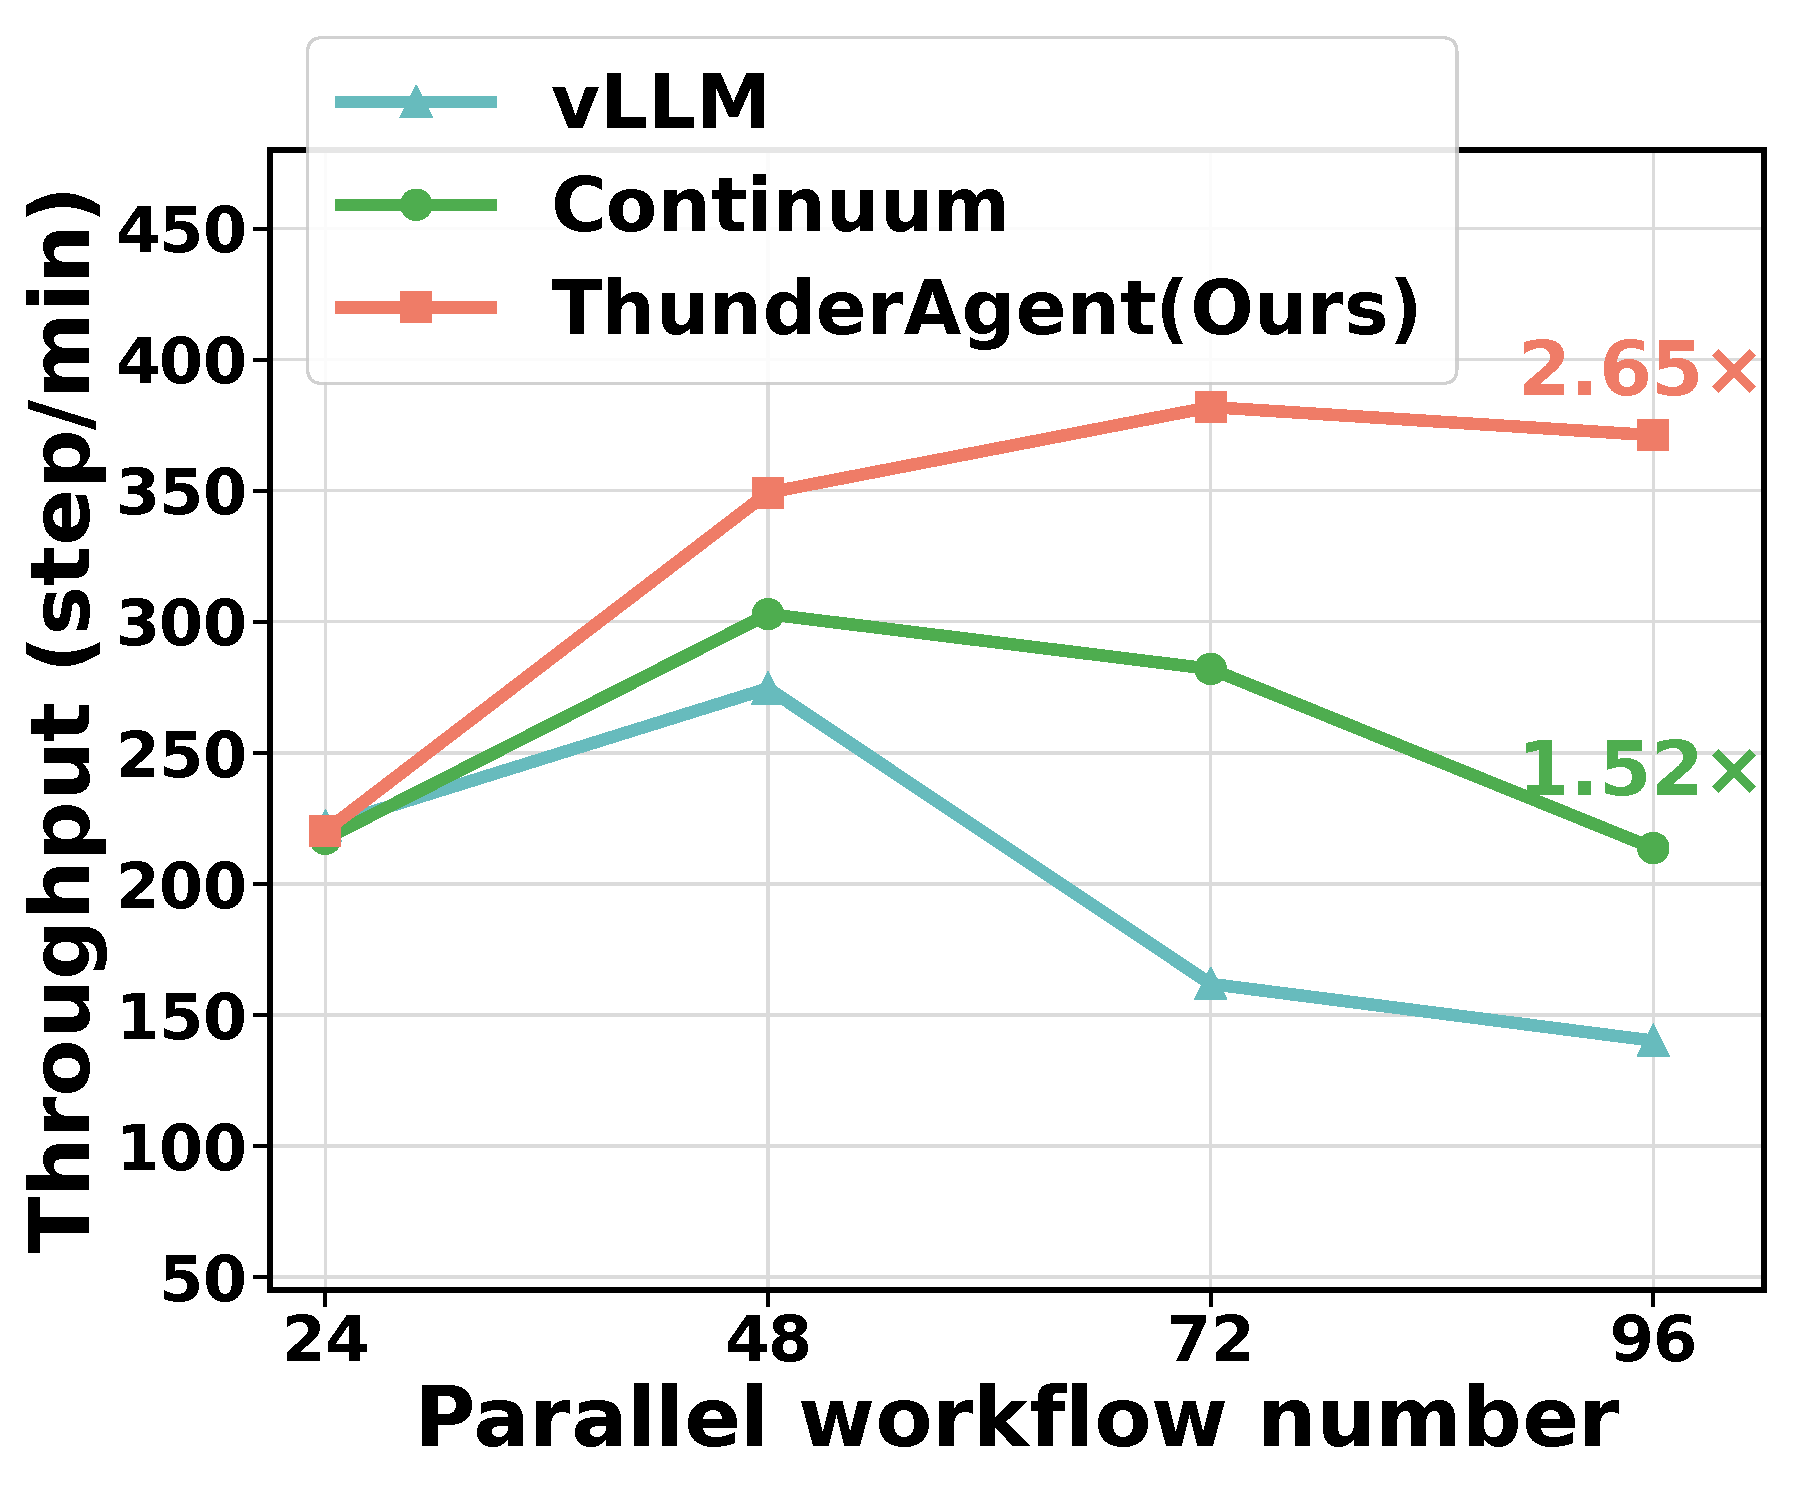
\includegraphics[width=\textwidth]{Figures/throughputs_vs_bs.pdf}  % 替换为你的图片路径
        \caption{吞吐量下降}
        \label{fig:throughputs_vs_bs}
    \end{subfigure}
    \begin{subfigure}{0.32\textwidth}
        \centering
        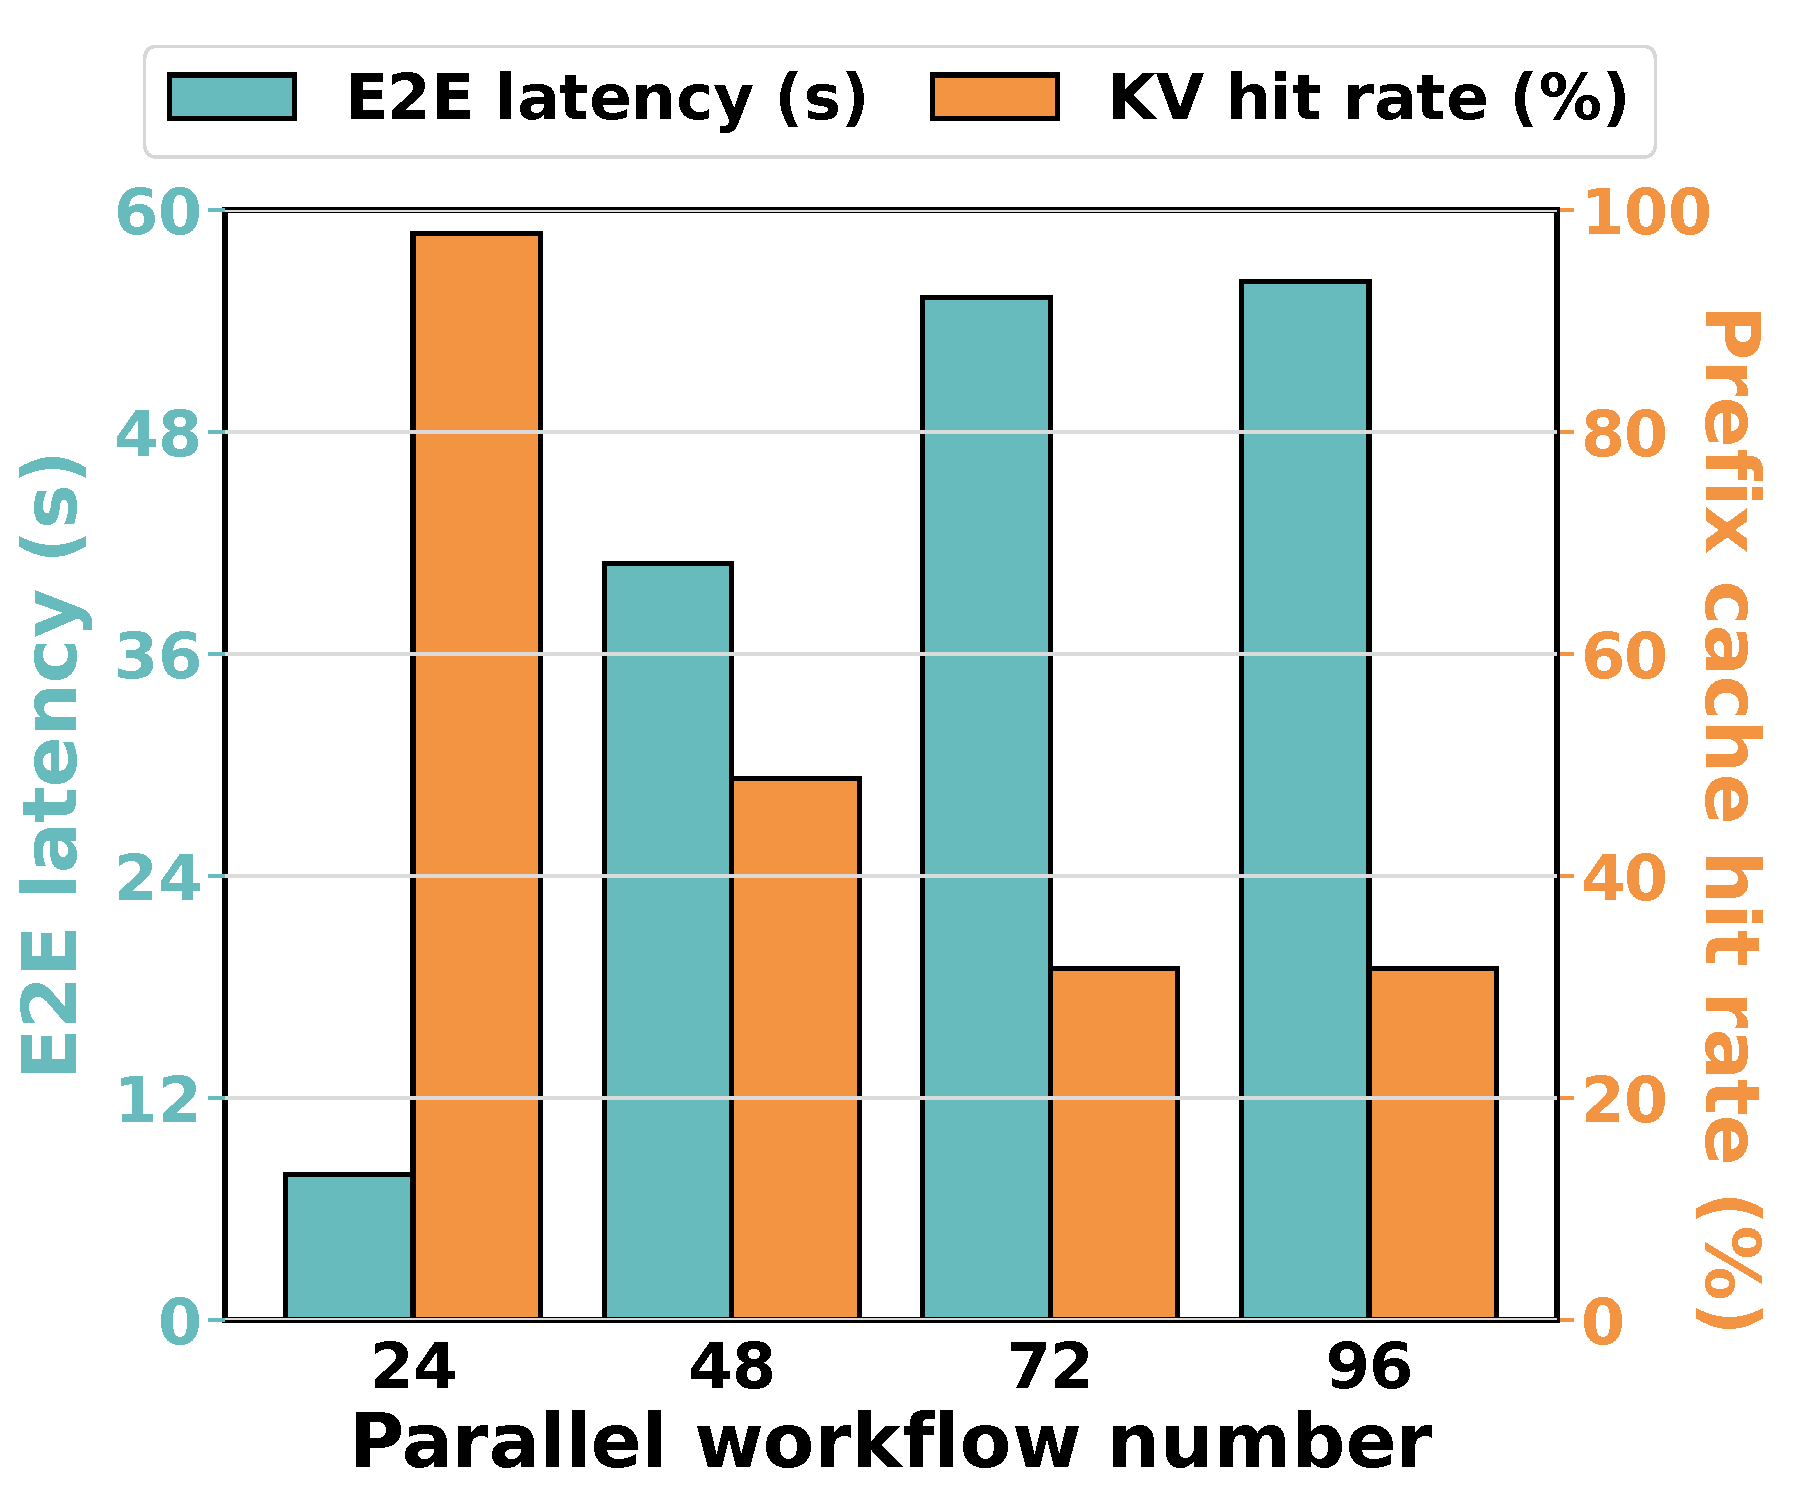
\includegraphics[width=\textwidth]{Figures/cachehit_latency_relation.pdf}  % 替换为你的图片路径
        \caption{KV 缓存抖动}
        \label{fig:workload_profile}
    \end{subfigure}
    \begin{subfigure}{0.32\textwidth}
        \centering
        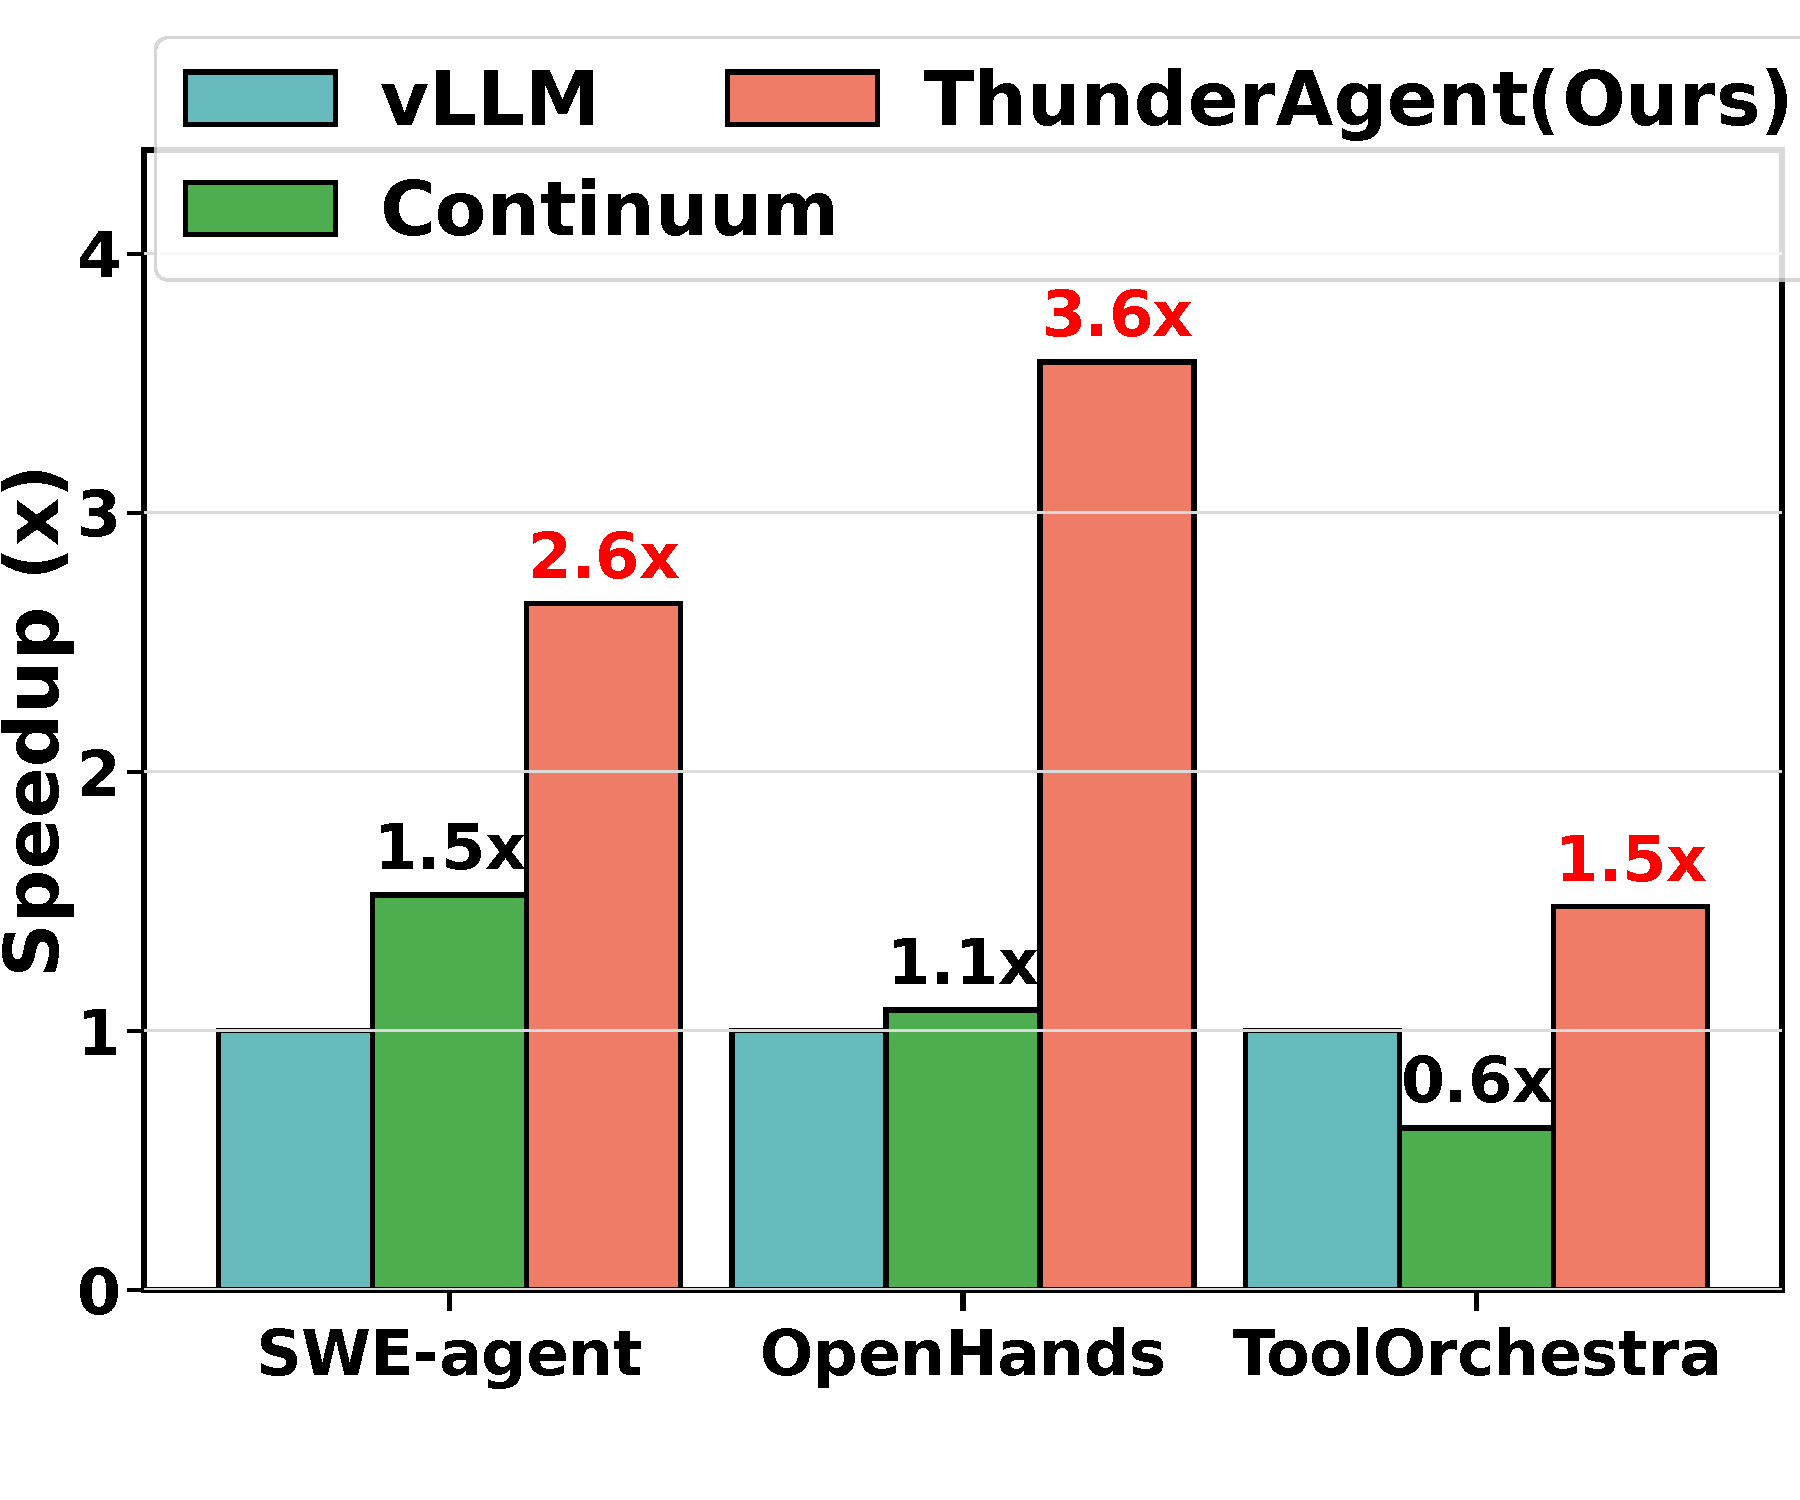
\includegraphics[width=\textwidth]{Figures/throughputs_compare.pdf}  % 替换为你的图片路径
        \caption{ 加速比 \ouralg}
        \label{fig:benefit}
    \end{subfigure}
    \caption{\textbf{随着并行工作流数量（即批量大小）增加，\ouralg 与既有智能体推理系统的性能比较。} 我们在 SWE-Bench Lite 上评估服务 SWE-Agent 的 GLM-4.6 MoE 模型（图 a 和 b），并在 8$\times$H100 GPU 集群上评估 SWE-Agent、OpenHands 和 ToolOrchestra（图 c）。结果表明：(a) 当前推理系统无法在大批量下保持高吞吐量；(b) 吞吐量下降主要源于较低的 KV 缓存命中率，这会增加端到端请求延迟；(c) 相比既有推理系统，\ouralg 通过减少 KV 缓存抖动并管理工具执行资源生命周期，实现了更高吞吐量。}
    \label{fig:three_subfigures}
    \vspace{-4mm}
\end{figure*}
语言模型的最新进展已将其用途从基础聊天机器人扩展到复杂智能体~\citep{yang2025qwen3technicalreport, 5team2025glm45agenticreasoningcoding}。
这些智能体通过将长链推理与外部工具调用（例如编译器、检索器）交错起来，解决编码~\citep{jimenez2024swebenchlanguagemodelsresolve,jain2024livecodebenchholisticcontaminationfree} 和计算机使用~\citep{xie2024osworldbenchmarkingmultimodalagents,bonatti2024windowsagentarenaevaluating} 等领域的现实问题，并且通常作为无需实时人工干预即可执行多步骤工作流的自主系统运行。
然而，现代推理系统的吞吐量会随着待处理智能体请求数量增加而下降（\autoref{fig:throughputs_vs_bs}）。与此同时，rollout 占强化学习（RL）总挂钟时间的 \textbf{70\%} 以上~\citep{Sheng_2025, fu2025areallargescaleasynchronousreinforcement}.
% S
% or reinforcement learning rollouts~\citep{hu2024openrlhf, yang2025dashinputawaredynamiclayer}

% Throughput degradation increases the cost and reduces the quality of agent inference systems. Unlike human-in-the-loop systems, where latencies are masked by user response times, agents operate autonomously. Coding and research agents execute long-running trajectories without requiring real-time human intervention. In these non-interactive workflows, maximizing throughput directly reducing the total serving cost by serving with less hardwares. Further, in asynchronous RL frameworks,
% low rollout throughput exacerbates policy lag—the weight discrepancy between training and rollout models, forcing the algorithm to learn from stale data and degrading convergence~\citep{fu2025areallargescaleasynchronousreinforcement, Sheng_2025, shenfeld2025rlsrazoronlinereinforcement,zheng2025stabilizingreinforcementlearningllms}.

随着智能体工作流在规模上越来越自治，整体系统效率更多由持续吞吐量决定，而不是像人机交互应用那样主要受尾延迟和用户响应时间支配。因此，更高吞吐量可以让硬件服务更多已完成工作流，从而直接降低服务成本。此外，在异步强化学习中，更高的 rollout 吞吐量可以减轻数据收集所用参数与正在更新的参数之间的策略滞后，使模型从陈旧性更低的数据中学习，进而提升收敛速度和最终策略质量~\citep{fu2025areallargescaleasynchronousreinforcement, Sheng_2025, shenfeld2025rlsrazoronlinereinforcement,zheng2025stabilizingreinforcementlearningllms}.


% The impact is even more severe in agentic reinforcement learning~\citep{hu2024openrlhf, yang2025dashinputawaredynamiclayer}, where rollout relies on extensive interaction with the environment and accounts for over 90\% of the total wall-clock time.
% Crucially, in asynchronous RL frameworks~\citep{fu2025areallargescaleasynchronousreinforcement, Sheng_2025},
% low rollout throughput exacerbates policy lag—the weight discrepancy between training and rollout models, forcing the algorithm to learn from stale data and significantly degrading convergence~\citep{shenfeld2025rlsrazoronlinereinforcement,zheng2025stabilizingreinforcementlearningllms}.

然而，当前智能体推理系统的吞吐量并不理想，因为它们通常由彼此隔离的组件松散组合而成：现成的模型推理引擎（例如 vLLM~\citep{kwon2023efficientmemorymanagementlarge} 或 SGLang~\citep{zheng2024sglangefficientexecutionstructured}）搭配通用工具编排器（例如 Kubernetes）。虽然智能体工作流涉及多轮模型请求和工具请求，这些组件仍在 \textit{按请求} 的层面分别调度和分配资源，缺少对整个工作流的端到端认知。这种设计带来了三个关键挑战：

\begin{enumerate}[itemsep=1pt,topsep=2pt,leftmargin=*]
\item
\textbf{KV 缓存抖动。} 请求感知系统在工具执行间隔期间过早地逐出 KV 缓存，而没有预见到智能体工作流中的未来重用。
因此，当工具调用完成时，系统需要重新运行预填充以恢复其整个交互历史记录。重新预填充成本会使智能体工作流的平均端到端延迟增加最多 \textbf{7.14$\times$} （看 \autoref{fig:workload_profile}）并降低吞吐量。

\item
\textbf{跨节点显存不均衡。} 请求感知引擎在多节点推理设置中存在利用率不平衡的问题。
% multi-turn agentic trajectories rapidly grow in sequence length causing high GPU memory pressure.
% Typically, routing all requests within a single workload to the same backend yields higher locality.
现有引擎将来自同一智能体工作流的所有请求固定到固定节点，以最大限度地提高 KV 缓存命中率。
然而，由于上下文长度在智能体工作流中快速且不可预测地扩展，
% this routing policy leads to memory imbalance across the cluster.
% it lacks the mechanism to transfer active agentic workloads between nodes. Consequently,
% S
在此路由策略下，一些节点达到了容量，而其他节点仍未得到充分利用。

\item
\textbf{工具生命周期的遗忘。}
% Most tool resources are shared across all requests within an agentic workload. However,
请求感知的编排器很难决定何时释放和准备工具执行所需的资源和环境。
% lack visibility into the workload lifecycle, these resources are often not released upon task termination.
因此，未使用的沙箱和 API 服务器继续占用关键磁盘空间和网络端口，导致资源累积耗尽和系统故障。
同时，智能体工作流在推理之前必须等待极长的设置时间。
% preparation are usually costly, and these parts could be prepared beforehand to improve end-to-end latency further.
\end{enumerate}

本文介绍 \ouralg，这是一种采用智能体工作流端到端视图的智能体推理系统，用于实现高吞吐量智能体服务和 RL rollout。
% rather than assembling fragmented request-level components.
% This framework enables the joint orchestration and optimization of LLM inference and tool lifecycles, moving beyond fragmented request-level management.
我们的具体贡献是：


% To establish a native serving infrastructure for agentic workflows, we introduce \ouralg, the first system to implement a program-level abstraction with a dedicated scheduler and garbage collector. The program scheduler provides the inference engine with visibility into tool-execution states, mitigating KV-cache thrashing and enabling cross-node program migration to maximize cluster throughput. Simultaneously, the lifecycle-aware garbage collector ensures the timely reclamation of tool resources and enables proactive environment initialization, significantly reducing resource overhead and end-to-end latency.

% \begin{enumerate}[itemsep=0.0pt,topsep=0pt,leftmargin=*]
%   \item \textbf{Program abstraction:} We model agent trajectories as persistent \textit{programs} spanning multiple model/tool steps and exposing semantic state (reasoning/acting/waiting) and resource metadata. This decouples scheduling from execution backends (e.g., vLLM/SGLang, Kubernetes), enabling easy integration of new tasks.

%   \item \textbf{Program-aware scheduler:} We formulate scheduling as constrained optimization to reduce re-prefill overhead and improve decoding throughput under GPU memory limits. We (i) pause tool-acting trajectories during memory pressure to protect reasoning KV cache, and (ii) migrate trajectories across DP nodes via a shared waiting queue to balance memory.

%   \item \textbf{Program-aware tool management:} We overlap I/O-heavy environment setup with LLM reasoning by tracking dependencies, and use termination signals to garbage-collect persistent tool resources (e.g., sandboxes, ports), preventing leaks and sustaining throughput.
% \end{enumerate}

% \junxiong{Is this part too long in abstraction? Should we just keep this a bit more high level, like this 1. We model agent trajectories as persistent \textit{programs} spanning multiple model/tool steps and exposing semantic state (reasoning/acting/waiting) and resource metadata. This decouples scheduling from execution backends (e.g., vLLM/SGLang), enabling easy integration of new tasks. 2. We formulate scheduling as constrained optimization to reduce re-prefill overhead and improve decoding throughput under GPU memory limits. We (i) pause tool-acting trajectories during memory pressure to protect reasoning KV cache, and (ii) migrate trajectories across DP nodes via a shared waiting queue to balance memory. 3. We overlap I/O-heavy environment setup with LLM reasoning by tracking dependencies, and use termination signals to clean up resources, preventing leaks and sustaining throughput.}



\begin{enumerate}[itemsep=0.0pt,topsep=0pt,leftmargin=*]

    \item \textbf{程序抽象：} 我们将智能体工作流抽象为 \textit{智能体程序}。
    智能体程序是一流的调度单元，它在多个模型调用和工具执行中持续存在，向运行时公开语义状态。
    程序跟踪工作流标识符、执行阶段（即推理或行动）、调度状态、总令牌和工具资源的元数据。这种抽象将调度与执行后端（例如 vLLM/SGLang）解耦，从而实现新工作流的无缝集成。
    % , and working status (active, paused).

    \item \textbf{程序感知调度器：} 基于程序抽象，我们将智能体推理调度视为约束优化问题，以最小化重新计算和缓存开销，并最大化预填充和解码吞吐量，具体取决于 GPU 显存容量。
    % We design a program-centric scheduler that utilizes the program metadata to resolve resource contention through
    我们引入两个关键机制：
    \begin{enumerate}[itemsep=0.0pt,topsep=0pt,leftmargin=*]
        \item \textbf{状态感知暂停：} 如果执行后端遇到显存压力，我们会通过工具调用选择性地暂停当前处于执行状态的工作流。这个设计有助于
        % the scheduler selectively suspends their execution
        为处于推理状态的程序保留内存，并消除任意的、次优的 KV 缓存驱逐。
        % that drive KV-cache thrashing.
        \item \textbf{动态迁移：} 我们跨数据并行 (DP) GPU 节点迁移智能体程序，以减轻显存不均衡。我们通过以下方式实现这一点
        % localized memory fragmentation by
        使所有 DP 节点共享一个全局程序感知等待队列，而不是强制来自程序的请求始终发送到同一节点。
        % Together, these mechanisms prevent systemic bottlenecks and inherently maximize aggregate throughput for both serving and RL rollout.
    \end{enumerate}

    \item \textbf{程序感知工具资源管理：} 在长期智能体工作负载中，工具环境是持久资源，其管理不善直接限制持续吞吐量。通过跟踪执行依赖性， \ouralg 将 I/O 密集型环境初始化与 LLM 推理重叠。
    % , eliminating the idle time caused by serialized bottlenecks.
    对于已完成的程序，我们实现了生命周期感知的垃圾收集器
    % that bridges the visibility gap between the inference engine and tool managers. By leveraging
    利用程序终止信号来回收工具资源，例如 Docker 沙箱和网络端口。
    % , such as Docker sandboxes and network ports.
    因此，这可以防止累积的资源泄漏并确保持续的高吞吐量智能体推理 \ouralg.

    % \item \textbf{Extensible Framework and Seamless Integration:} The program-level abstraction provides a unified interface for ReAct-based workflows. By decoupling agent logic from the execution layer, \ouralg enables seamless integration with request-centric backends (e.g., vLLM and SGLang) and orchestrators (e.g., Kubernetes), requiring minimal engineering effort to support new agentic tasks.
\end{enumerate}

上述贡献无法在请求感知推理引擎中实现。如果没有程序状态和工作流依赖性的显式表示，请求感知调度器无法区分临时工具等待和终止，也无法将 GPU 显存与程序级资源调度协调起来。

% We evaluate \ouralg across diverse serving and rollout scenarios, including code agents such as SWE-agent~\citep{yang2024sweagentagentcomputerinterfacesenable} and OpenHands~\citep{wang2025openhandsopenplatformai}, and tool-use agents like ToolOrchestra. Our experiments span SWE-bench~\citep{jimenez2024swebenchlanguagemodelsresolve}, and HLE-bench~\citep{phan2025humanitysexam}, with model scales ranging from 8B Qwen3~\citep{yang2025qwen3technicalreport} to 355B GLM-4.6 MoE~\citep{5team2025glm45agenticreasoningcoding}. Conducted on RTX 5090 and H100 GPU clusters, these evaluations demonstrate that \ouralg achieves \textbf{1.48--3.58$\times$} throughput improvements shown in \autoref{fig:benefit}.

% The program-level abstraction provides a unified interface for ReAct-based workflows.
我们评估 \ouralg 跨不同的智能体工作负载。为了 \textbf{服务}，我们评估 ToolOrchestra~\citep{su2025toolorchestraelevatingintelligenceefficient} 作为 HLE-Bench 上的路由智能体~\citep{phan2025humanitysexam}，SWE-Agent~\citep{yang2024sweagentagentcomputerinterfacesenable} 以及OpenHands~\citep{wang2025openhandsopenplatformai} 作为 SWE-bench 上的编码智能体~\citep{jimenez2024swebenchlanguagemodelsresolve}，以及 OpenHands 作为 ScienceAgentBench 上的科学发现智能体~\citep{chen2024scienceagentbenchrigorousassessmentlanguage}，实现 \textbf{1.48--3.58$\times$} 吞吐量改进如图所示 \autoref{fig:benefit}。为了 \textbf{强化学习 rollout}，我们进一步在分布式 GPU 节点上测试编码智能体，实现  \textbf{1.79--3.92$\times$} 与之前的 SOTA 系统相比有所改进。

% We evaluate \ouralg across diverse agentic workloads, including \textbf{RL rollouts and serving} for coding agents such as SWE-Agent~\citep{yang2024sweagentagentcomputerinterfacesenable} and OpenHands~\citep{wang2025openhandsopenplatformai}, alongside \textbf{standard serving} for tool-use agents like ToolOrchestra~\citep{su2025toolorchestraelevatingintelligenceefficient}. Our experiments span SWE-bench~\citep{jimenez2024swebenchlanguagemodelsresolve} and HLE-bench~\citep{phan2025humanitysexam}, with model scales ranging from 8B Qwen3~\citep{yang2025qwen3technicalreport} to 355B GLM-4.6 MoE~\citep{5team2025glm45agenticreasoningcoding}. We conduct experiments on RTX 5090 and H100 GPU clusters, demonstrating that \ouralg achieves \textbf{1.48--3.58$\times$} throughput improvements across settings, shown in \autoref{fig:benefit}.

% We also implemented our system at a leading ai inference company to speed up their coding agent RL training workload by \textbf{2.31$\times$} in total.


% However, current agent serving systems are not designed to satisfy such throughput demands.

% Most agentic serving frameworks are constructed by assembling independent resource management tools, typically coupling request-level serving engines like vLLM~\citep{kwon2023efficientmemorymanagementlarge} and SGLang~\citep{zheng2024sglangefficientexecutionstructured} with general-purpose tool schedulers like Kubernetes. This architecture presents a granularity misalignment: serving engines are optimized for stateless, independent requests, utilizing KV-cache eviction policies like Least Recently Used (LRU) to maximize instantaneous GPU utilization. Consequently, these systems treat the interval of external tool execution as a session termination or generic idleness, ignoring the agent's requirement to persist context for subsequent steps. This leads to premature KV-cache eviction: when the tool execution concludes, the system is forced to re-prefill the full history, leading to massive cache misses and causing significant computational overhead. \autoref{fig:workload_profile} shows that request-level infrastructures failed to maintain high throughputs in large batch serving due to heavy re-prefill latency. While recent schedulers like Continuum~\citep{li2025continuumefficientrobustmultiturn} attempt to address this via predictive pinning, they rely on the assumption of deterministic tool durations. In agentic workflows like Tool Orchestra~\citep {su2025toolorchestraelevatingintelligenceefficient} and GPU Kernel Scientist~\citep{andrews2025gpukernelscientistllmdriven} that interact with complex environments, however, tool execution times are inherently variable, making prediction-based mechanisms difficult to stabilize in practice.

% \yinfang{I like this paragraph, but it can be written better by providing more details.}



% Furthermore, the absence of a unified program abstraction prevents the coordinated management of heterogeneous resource lifecycles under stochastic workloads. Specifically, the lifecycle of the GPU resource operates independently from its tools and environment (Docker/Sandbox). This disjoint management leads to inefficient resource reclamation, where "zombie" tools like sandboxes persist in memory and disk after an agent has finished or stalled, limiting the scheduling of new tasks.

% Large Language Models (LLMs) have demonstrated exceptional performance in single-turn generation tasks, such as mathematical reasoning and question answering.
% However, solving composite real-world problems requires extending these capabilities to multi-turn interactions, where the model must maintain persistent context across extended sessions.
% This paradigm is further expanded in agentic workflows.
% Notably, the ReAct framework has emerged as the \textit{de facto} standard for constructing such systems.
% By interleaving multi-step reasoning with the execution of \textbf{heterogeneous external tools}, such as compilers, terminals, and remote APIs, ReAct agents can autonomously accomplish composite tasks[cite: 4, 10].

% However, this transition comes with an throughputs Degradation on infrastructure. Executing these long-lived, multi-turn programs consumes vast inference budgets, not just in GPU compute and memory, but across heterogeneous resources including costly remote model APIs, CPU and disk I/O for sandbox and retriever.
% Our empirical analysis reveals a startling gap: compared to single-turn code generation benchmarks BigCode Bench, running multi-turn agentic workloads, OpenHands, results in over \textbf{9.7$\times$ throughput degradation} and consumes massive storage, over \textbf{6TB} of disk usage in our large-scale stress tests.

% This throughput degradation constitutes a fundamental bottleneck for autonomous agentic systems.
% Unlike human-in-the-loop applications, where system latency is masked by user response time, agents operate continuously and autonomously.
% Consequently, system throughput directly dictates the feasibility of large-scale evaluation(e.g., running SWE-bench on thousands of instances) and the cost-efficiency of deployment[cite: 7, 8].
% This bottleneck is even more pronounced in Agentic Reinforcement Learning (RL), where rollout relies on extensive interaction with the environment.
% Studies indicate that this rollout phase dominates the training budget, accounting for over 83\% of the total wall-clock time.

% Crucially, in asynchronous RL frameworks, low rollout throughput exacerbates the latency between data generation and model updates, increasing the divergence between the rollout policy and the training policy (policy lag).
% Thus, maintaining high throughput of large batch serving and rollout is a prerequisite for both efficient serving and stable RL training.


% Crucially, in asynchronous training frameworks, low rollout throughput exacerbates the "policy lag"—the weight difference between the training model and the rollout model. This latency forces the algorithm to learn from stale, off-policy data, significantly degrading convergence speed and accuracy. Thus, maintaining high throughput in large-batch scenarios is a prerequisite for effective Agentic RL.

% Current infrastructure is not designed to satisfy agentic throughput demands.
% Most agentic serving frameworks are constructed by assembling independent resource management tools, typically coupling request-level serving engines (e.g., vLLM, SGLang) with general-purpose tool schedulers (e.g., Kubernetes, retriever server).


% This architecture presents a \textbf{granularity misalignment}: serving engines are optimized for stateless, independent requests, utilizing KV cache eviction policies like Least Recently Used (LRU) to maximize instantaneous GPU utilization.
% Consequently, these systems treat the interval of external tool execution as a session termination or generic idleness, ignoring the agent's requirement to persist context for subsequent steps.
% This leads to premature KV-cache eviction: when the tool execution concludes, the system is forced to re-pefill the full history, leading to huge KV cache missrate and causing significant computational overhead and throughput degradation[cite: 36, 41, 42].

% Furthermore, this lack of a unified program-level view fail to manage the \textbf{coupled lifecycles} of heterogeneous resources in the face of workload stochasticity.
% Specifically, the lifecycle of the GPU resource operates independently from its tools and environment (Docker/Sandbox).
% This disjoint management could lead to unefficient garbage collection, where sandboxes persist in memory and disk after an agent has finished or stalled—limiting the scheduling of new tasks.
% While recent schedulers like Continuum address preemption via predictive pinning, they rely on the assumption of deterministic tool durations. However, pinned KV caches could still be evicted in extreme heavy workloads. And in complex agentic workflows, tool execution times are inherently variable (e.g., dependent on network I/O or search depth), making such prediction-based mechanisms difficult to stabilize in practice.

% Furthermore, this lack of a unified program-level view affects heterogeneous resource orchestration.
% In current systems, the lifecycle of the GPU resource operates independently from its tool and environment (Docker/Sandbox).
% This separation often leads to \textbf{"Zombie" containers}—where sandboxes persist in memory and disk after an agent has finished or stalled—limiting the scheduling of new tasks.
% While recent schedulers like Continuum address this via predictive pinning, they assume deterministic tool durations.
% However, in complex agentic workflows, tool execution times are variable, making prediction-based pinning difficult to stabilize in practice.

% To bridge this gap, we present \textbf{ThunderReact}, a program-centric infrastructure designed specifically for the efficient serving and rollout of stateful agentic systems. Unlike prior works that optimize components in isolation, ThunderReact treats the agent program as the first-class scheduling entity, orchestrating the end-to-end lifecycle of both neural and symbolic resources. Through our experiments on various agent tasks and models, our method have show no throughput degradation in large batch serving and rollout with 3$\times$ improvements compared with request level serving engine and 4$\times$ disk memory saving with tool optimizations. Our specific contributions are:

% \begin{itemize}
%     \item \textbf{Program-Centric Abstraction and Infrastructure:} We formalize the agentic task as a program, a continuous scheduling entity that encapsulates both GPU and other heterogeneous resources. Based on this abstraction, we architect a unified infrastructure designed to synergistically optimize the execution of complex agentic tasks. By implementing a feedback-based congestion control mechanism that minimizes the \textit{Resource-Time Product}[cite: 89, 91], our system maintains high throughputs and is cost-efficient for agentic serving and rollout.

%     \item \textbf{Multi-Node Program-Level Scheduler:} We design a distributed scheduler to address memory imbalance and preemption challenges in multi-node serving and rollout. By tracking the memory footprint and execution stage of each program, our system transforms rigid load balancing (or simple KV-aware routing) into \textbf{dynamic stateful placement}. This mechanism enables \textbf{collaborative preemption and active migration}, where programs on congested nodes are proactively paused and moved to underutilized workers. This dynamic re-balancing effectively resolves hot-spots and prevents head-of-line blocking caused by long-context agents.

%     \item \textbf{Lifecycle-Coupled Resource Optimization:} We implement fine-grained resource management for heterogeneous tools, featuring program-aware garbage collection and request-level micro-batching[cite: 147, 149]. By coupling the lifecycle of Docker sandboxes with the agent program, we ensure immediate resource reclamation upon task completion. Furthermore, our micro-batching strategy for tool execution mitigates I/O contention during large-batch rollouts, preventing system overload from concurrent external requests.
% \end{itemize}





% 1. LLM agents are transfering single turn generation to multiple generations with tool call. (Introduce react agent, \textbf{single turn -> multiturn turn -> multiturn with outside multiple resource}) Do we need a figure of react agent? We do not need it just use words to describe. An example figure
% % \textbf{显示不是单一LLM而是多方面的tools}
% 2. These agents are very expensive in evaluate and rollout. (figure 1 here, x-axis parallel task number?, y-axis average program execution time with prefill/decode/tool call ratio). \textbf{One sentence is enough, there is no need to put a graph} No figure here.

% 3. In such senarios, throughputs is the most important figure for efficiency. Current request level serving engine vllm. sglang failed to work well at large batch evaluation RL. (figure 1 here, x-axis is parallel task number, y-axis is throughput(step/min? token/s?))
% % \textbf{现在serving engine没有考虑programing level的关系，问题出在很多层面比如disk/cpu/GPU一个最主要的例子是GPU memory contention}
% 4. This is because KV cache is program level resource. multiturn task will preempt each other and make kv hit rate really slow and cause reprefill. (Figure3 here, x-axis parallel task number, y-axis KV cache hit rate)
% % Hetergenious system, 管理LLM，管理tool，管理所有事情。强调Disk usage，要讲的大一点，vllm + program没办法解决全部的问题。

% 4. Our contribution
%     1) Program level congestion control
%     2) multinode program-level scheduler
%     3) program-level outside reousce life cycle control and large batch optimization.
